\documentclass[10pt,twoside,reqno]{book}
\usepackage[utf8]{inputenc}
\usepackage[marginparsep=1em]{geometry}
\geometry{lmargin=.50in,rmargin=.50in, tmargin=0.75in, bmargin=0.75in}
\usepackage[english]{babel}
\usepackage{indentfirst}
\usepackage{amsfonts}
\usepackage{amscd}
\usepackage{amsthm}
\usepackage{amssymb}
\usepackage{amsmath}
\usepackage{accents}
\usepackage{graphicx}
\usepackage{enumitem}
\usepackage{lettrine}
\usepackage{slashed}
\usepackage{tikz}
\usepackage{fancyhdr}
\usepackage[hidelinks]{hyperref}
\usepackage{cancel}
\renewcommand{\qedsymbol}{$\blacksquare$}

\newtheorem{innercustomgeneric}{\customgenericname}
\providecommand{\customgenericname}{}
\newcommand{\newcustomtheorem}[2]{%
		\newenvironment{#1}[1]{%
		\renewcommand\customgenericname{#2}%
		\renewcommand\theinnercustomgeneric{##1}%
		\innercustomgeneric
		}{\endinnercustomgeneric}
}
\newcustomtheorem{customthm}{Theorem}
\newcustomtheorem{customlemma}{Lemma}
\newcustomtheorem{customdefinition}{Definition}
\newcustomtheorem{customcoro}{Corollary}
\newcustomtheorem{customexa}{Example}
\newcustomtheorem{cusques}{Question}


\newcommand{\R}{\mathbb{R}}
\newcommand{\B}{\mathcal{B}}
\newcommand{\ds}{\displaystyle}
\newcommand{\h}{homeomorphism}
\newcommand{\hs}{homeomorphisms}
\newcommand{\Hs}{Homeomorphisms}
\newcommand{\hc}{homeomorphic}
\newcommand{\widesim}[2][1.5]{
\mathrel{\overset{#2}{\scalebox{#1}[1]{$\sim$}}}
}

\pagestyle{fancy}
\fancyhf{}
\lhead{\hyperlink{toc}{Clay Mathematics}}
\fancyfoot[L,RO]{Xiang Gao}
\fancyfoot[R,RO]{\hyperlink{toc}{Table of Contents}}
\rhead{\thepage}
\renewcommand{\footrulewidth}{0.4pt}

\title{Glossary for Topology\\\begin{center}
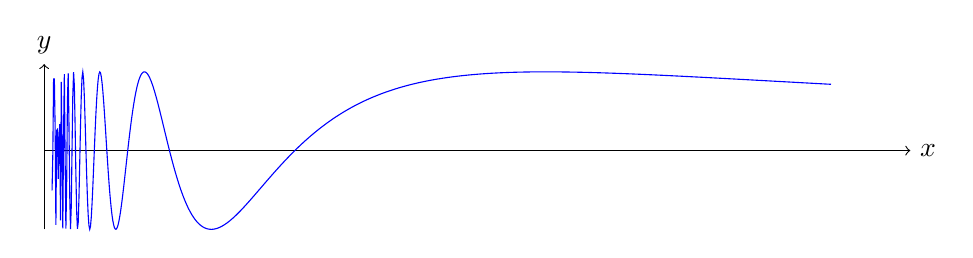
\begin{tikzpicture}[x=10cm]
        \draw[->] (0,0) -- (1.1,0) node[right] {$x$};
        \draw[->] (0,-1) -- (0,1.1) node[above] {$y$};
        \draw[blue,domain=0.01:1,samples=1000] plot (\x, {sin((1/\x)r)});
\end{tikzpicture}
\end{center}}
\author{Xiang Gao}